\documentclass[tikz,border=4pt]{standalone}
\usepackage[T1]{fontenc}
\usetikzlibrary{arrows.meta,positioning}

\definecolor{CompassBlue}{HTML}{284B63}
\definecolor{CompassLight}{HTML}{EDF3F6}
\definecolor{CompassWarm}{HTML}{F7F1E8}
\definecolor{CompassGray}{HTML}{5C6670}

\tikzset{
  box/.style={draw=CompassBlue, rounded corners=1.5pt, align=center,
              inner sep=2.4pt, minimum height=7mm, line width=0.65pt,
              font=\sffamily\scriptsize},
  source/.style={box, fill=CompassLight, text width=27mm},
  path/.style={box, text width=30mm},
  result/.style={box, fill=CompassWarm, text width=25mm},
  analysis/.style={draw=CompassGray, dashed, rounded corners=1.5pt,
                   align=center, inner sep=2.4pt, text width=76mm,
                   line width=0.6pt, font=\sffamily\scriptsize},
  flow/.style={-{Stealth[length=1.6mm]}, line width=0.7pt,
               draw=CompassBlue},
  offline/.style={-{Stealth[length=1.6mm]}, line width=0.65pt,
                  dashed, draw=CompassGray}
}

\begin{document}
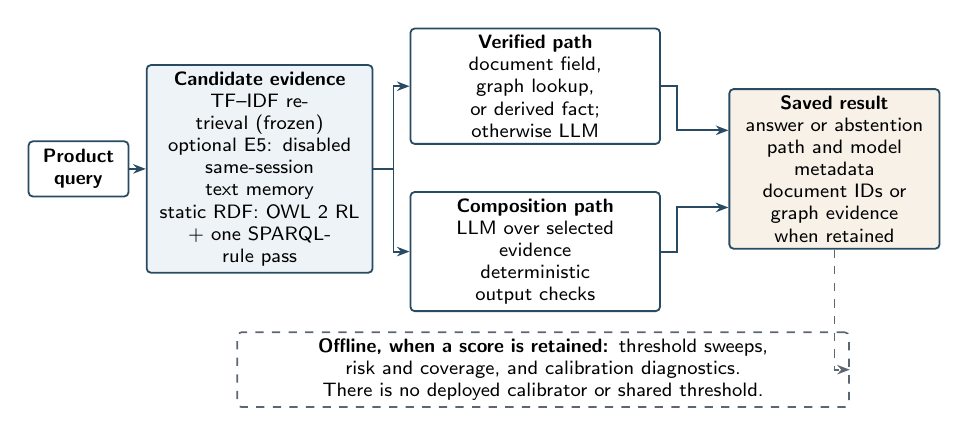
\begin{tikzpicture}
  \node[box, text width=11mm] (query) at (0.65,0)
    {\textbf{Product\\query}};

  \node[source] (evidence) at (2.95,0)
    {\textbf{Candidate evidence}\\
     TF--IDF retrieval (frozen)\\
     optional E5: disabled\\
     same-session text memory\\
     static RDF: OWL 2 RL\\
     + one SPARQL-rule pass};

  \node[path] (verified) at (6.45,1.05)
    {\textbf{Verified path}\\
     document field, graph lookup,\\
     or derived fact; otherwise LLM};

  \node[path] (composition) at (6.45,-1.05)
    {\textbf{Composition path}\\
     LLM over selected\\evidence\\
     deterministic output checks};

  \node[result] (saved) at (10.25,0)
    {\textbf{Saved result}\\
     answer or abstention\\
     path and model metadata\\
     document IDs or graph evidence\\
     when retained};

  \node[analysis] (posthoc) at (6.55,-2.55)
    {\textbf{Offline, when a score is retained:}
     threshold sweeps, risk and coverage, and calibration diagnostics.\\
     There is no deployed calibrator or shared threshold.};

  \draw[flow] (query.east) -- (evidence.west);
  \coordinate (split) at (4.65,0);
  \draw[flow] (evidence.east) -- (split) |- (verified.west);
  \draw[flow] (evidence.east) -- (split) |- (composition.west);
  \draw[flow] (verified.east) -- (8.25,1.05) |- (saved.160);
  \draw[flow] (composition.east) -- (8.25,-1.05) |- (saved.200);
  \draw[offline] (saved.south) |- (posthoc.east);
\end{tikzpicture}
\end{document}
